% \chapter{Design}
In this chapter, we discuss the design of the individual MONDRIAN components, as well as what design changes we come up with to make the MONDRIAN version more suitable for the data center environment. In particular, we have a look at the design of the MONDRIAN Controller, the Endpoint \acs{TP} and the Gateway \acs{TP}.


\subsection{MONDRIAN Controller}
Regarding the MONDRIAN Controller, we don't introduce any new concepts. Meaning that design wise it is identical to the MONDRIAN Controller from the original MONDRIAN design. This is useful since like this we can seamlessly combine traditional MONDRIAN deployments with the adapted version, which is designed specifically for data centers.

However, some details have not been fully specified in the original MONDRIAN design and are therefore worth pointing out. The current \acs{PoC} (\acl{PoC}) implementation of the current MONDRIAN Controller doesn't support the policies as described in the paper \cite{kwonmondrian} but instead just matches the source and destination zones. In our design however, we consider the full 5-tuplet as described in formula \ref{policy} and allow all fields to be wildcards. As protocols, we consider the transport layer protocols \acs{UDP} and \acs{TCP}. Furthermore, since we secure the control plane traffic between the MONDRIAN Controller and the Gateway \acs{TP} and the Endpoint \acs{TP} using asymmetric cryptography, we assume that we have a standard \acs{PKI} in place, which handles the distribution of the certificates. In our implementation we however just simulate the \acs{PKI} by previously distributing the certificates, just like it is done in the \acs{PoC} implementation of the original MONDRIAN.

%\todo{ \\
%    - Left as in the original design \\
%    - Implementation also considers wildcards and full 5-tuplet \\
%    - Communication secured with asymmetric crypto
%}
\subsection{Endpoint TP}
The Endpoint \acs{TP} is designed to be an application, which is running on top of an \acs{SDN} controller. It employs a reactive \acs{SDN} strategy, meaning that the first packet of a new flow will generate a packet-in message, which is sent to the \acs{SDN} controller. On the \acs{SDN} controller, there will be a processing pipeline, where packet-in handlers of different applications will process the packet-in message sequentially. Since an Endpoint \acs{TP} only allows or disallows traffic, it should be placed first in the \acs{SFC}. This means that the \acs{SDN} controller has to ensure that the Endpoint \acs{TP}'s packet-in handler is processed first. 

When a packet-in message is processed by an Endpoint TP, it first must parse the necessary header information such as the source and destination address, the source and destination port as well as the transport layer protocol. Then it will query the Transfer Module, where the packet is matched against the policies relevant for this site. Based on the outcome of this check, the Endpoint \acs{TP} then installs a flow table entry on the switch that generated the packet-in message. This means that following packets of this flow won't generate new packet-in messages for as long as the flow table entry didn't expire. To preserve the order of the \acs{SFC} on the \acs{SDN} switches, different \acs{SDN} applications are typically implemented in different flow tables. Since the Endpoint \acs{TP} is supposed to be the first service, it will install its flow table entries in flow table zero. The next service (e.g. a learning switch) will be implemented in flow table one. If an Endpoint \acs{TP} allows a flow, then the action will simply be a \texttt{GotoTable(1)} action, which allows the second service in the \acs{SFC} to process the packet. If the Endpoint \acs{TP} decides to drop a packet, then the OpenFlow action will be a \texttt{drop}, meaning that no subsequent service will be allowed to process the packet. 

It is worth pointing out that such a design has the benefit that only a fraction of all packets need to be processed by the Endpoint \acs{TP} application while most packets are forwarded or dropped very efficiently by the \acs{SDN} switches. This offers the Endpoint \acs{TP} the scalability and performance that is needed in modern data centers.
%todo{ \\
%   - App based on SDN Controller \\
%   - Explain Service Function Chaining using flow tables and chaining packet-in handlers \\
%   - Explain why reactive approach was chosen \\
%   - Explain what parts are handled by the switch and what by the Endpoint TP app 
%
\subsection{Gateway TP}
At the Gateway \acs{TP} the conversion between \acs{IP} and MONDRIAN packets takes place. Since the payload of a MONDRIAN packet is the encrypted original \acs{IP} packet, the Gateway \acs{TP} needs to be powerful enough to perform line-rate encryption and decryption. Such costly operations can't be handled by a simple \acs{SDN} switch but instead require more powerful hardware, ideally supporting hardware accelerated cryptographic operations such as the \acs{AES-NI} (\acl{AES-NI}) instruction \cite{rott2012AESNI}.

We therefore design the Gateway \acs{TP} as a traditional middlebox. However, we still need to ensure that it integrates into the highly virtualized environment that we find in a data center. Therefore, we design the Gateway \acs{TP} to be a \acs{VM}/container-based \acs{VNF}. \aclp{VM} can perform line-rate cryptographic operations, as we can see when we consider virtualized \acs{VPN} servers.

Deploying a Gateway \acs{TP} in a \acs{VM} or in a container allows us to quickly spin up/down new instances of a Gateway \acsp{TP} as the demand increases or decreases. Especially containers can be started and stopped within seconds. 

Another advantage of the new design is that the Gateway \acs{TP} is no longer in charge of authorizing zone transitions, meaning that it can be kept leaner and can therefore be implemented more efficiently than the original \acsp{TP}. At the same time it only has to deal with inter-domain traffic (see figure \ref{DC MONDRIAN Overview}), meaning that a Gateway \acs{TP} will be able to handle more hosts than a traditional \acs{TP}. 

\begin{figure}[t]
	\centering
	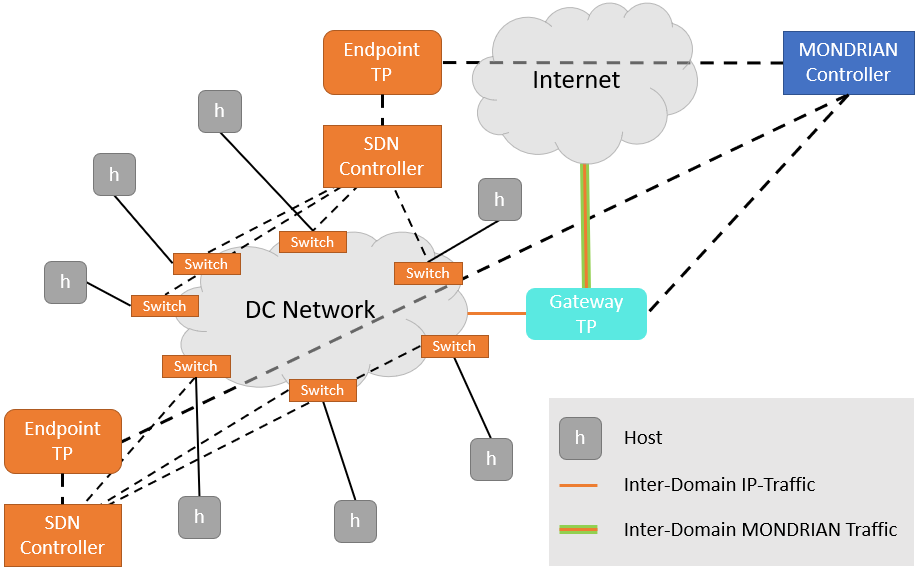
\includegraphics[width =0.48\textwidth]{img/DC_Mondrian_overview2.png}
	\caption{\acs{DC} (\acl{DC}) MONDRIAN Overview}
	\label{DC MONDRIAN Overview}
\end{figure}

%\todo{ \\
%    - Encryption/Decryption requires more advanced hardware than Switches \\
%    - Virtual middlebox can provide line-rate crypto \\
%    - Deploying it as VMs makes scalability easy -- spin up more if needed \\
%    - High performance implies that only the essential tasks should performed there (move authorization into the Endpoint TPs)
%}